\newpage
\section{$NO_x$ process model derivation from governing equations}
The discrete nonlinear recursive model that is linear in parameters can be derived from the molar conservation equations directly. The model derivation involves three main steps:
\begin{figure}[H]
        \centering
        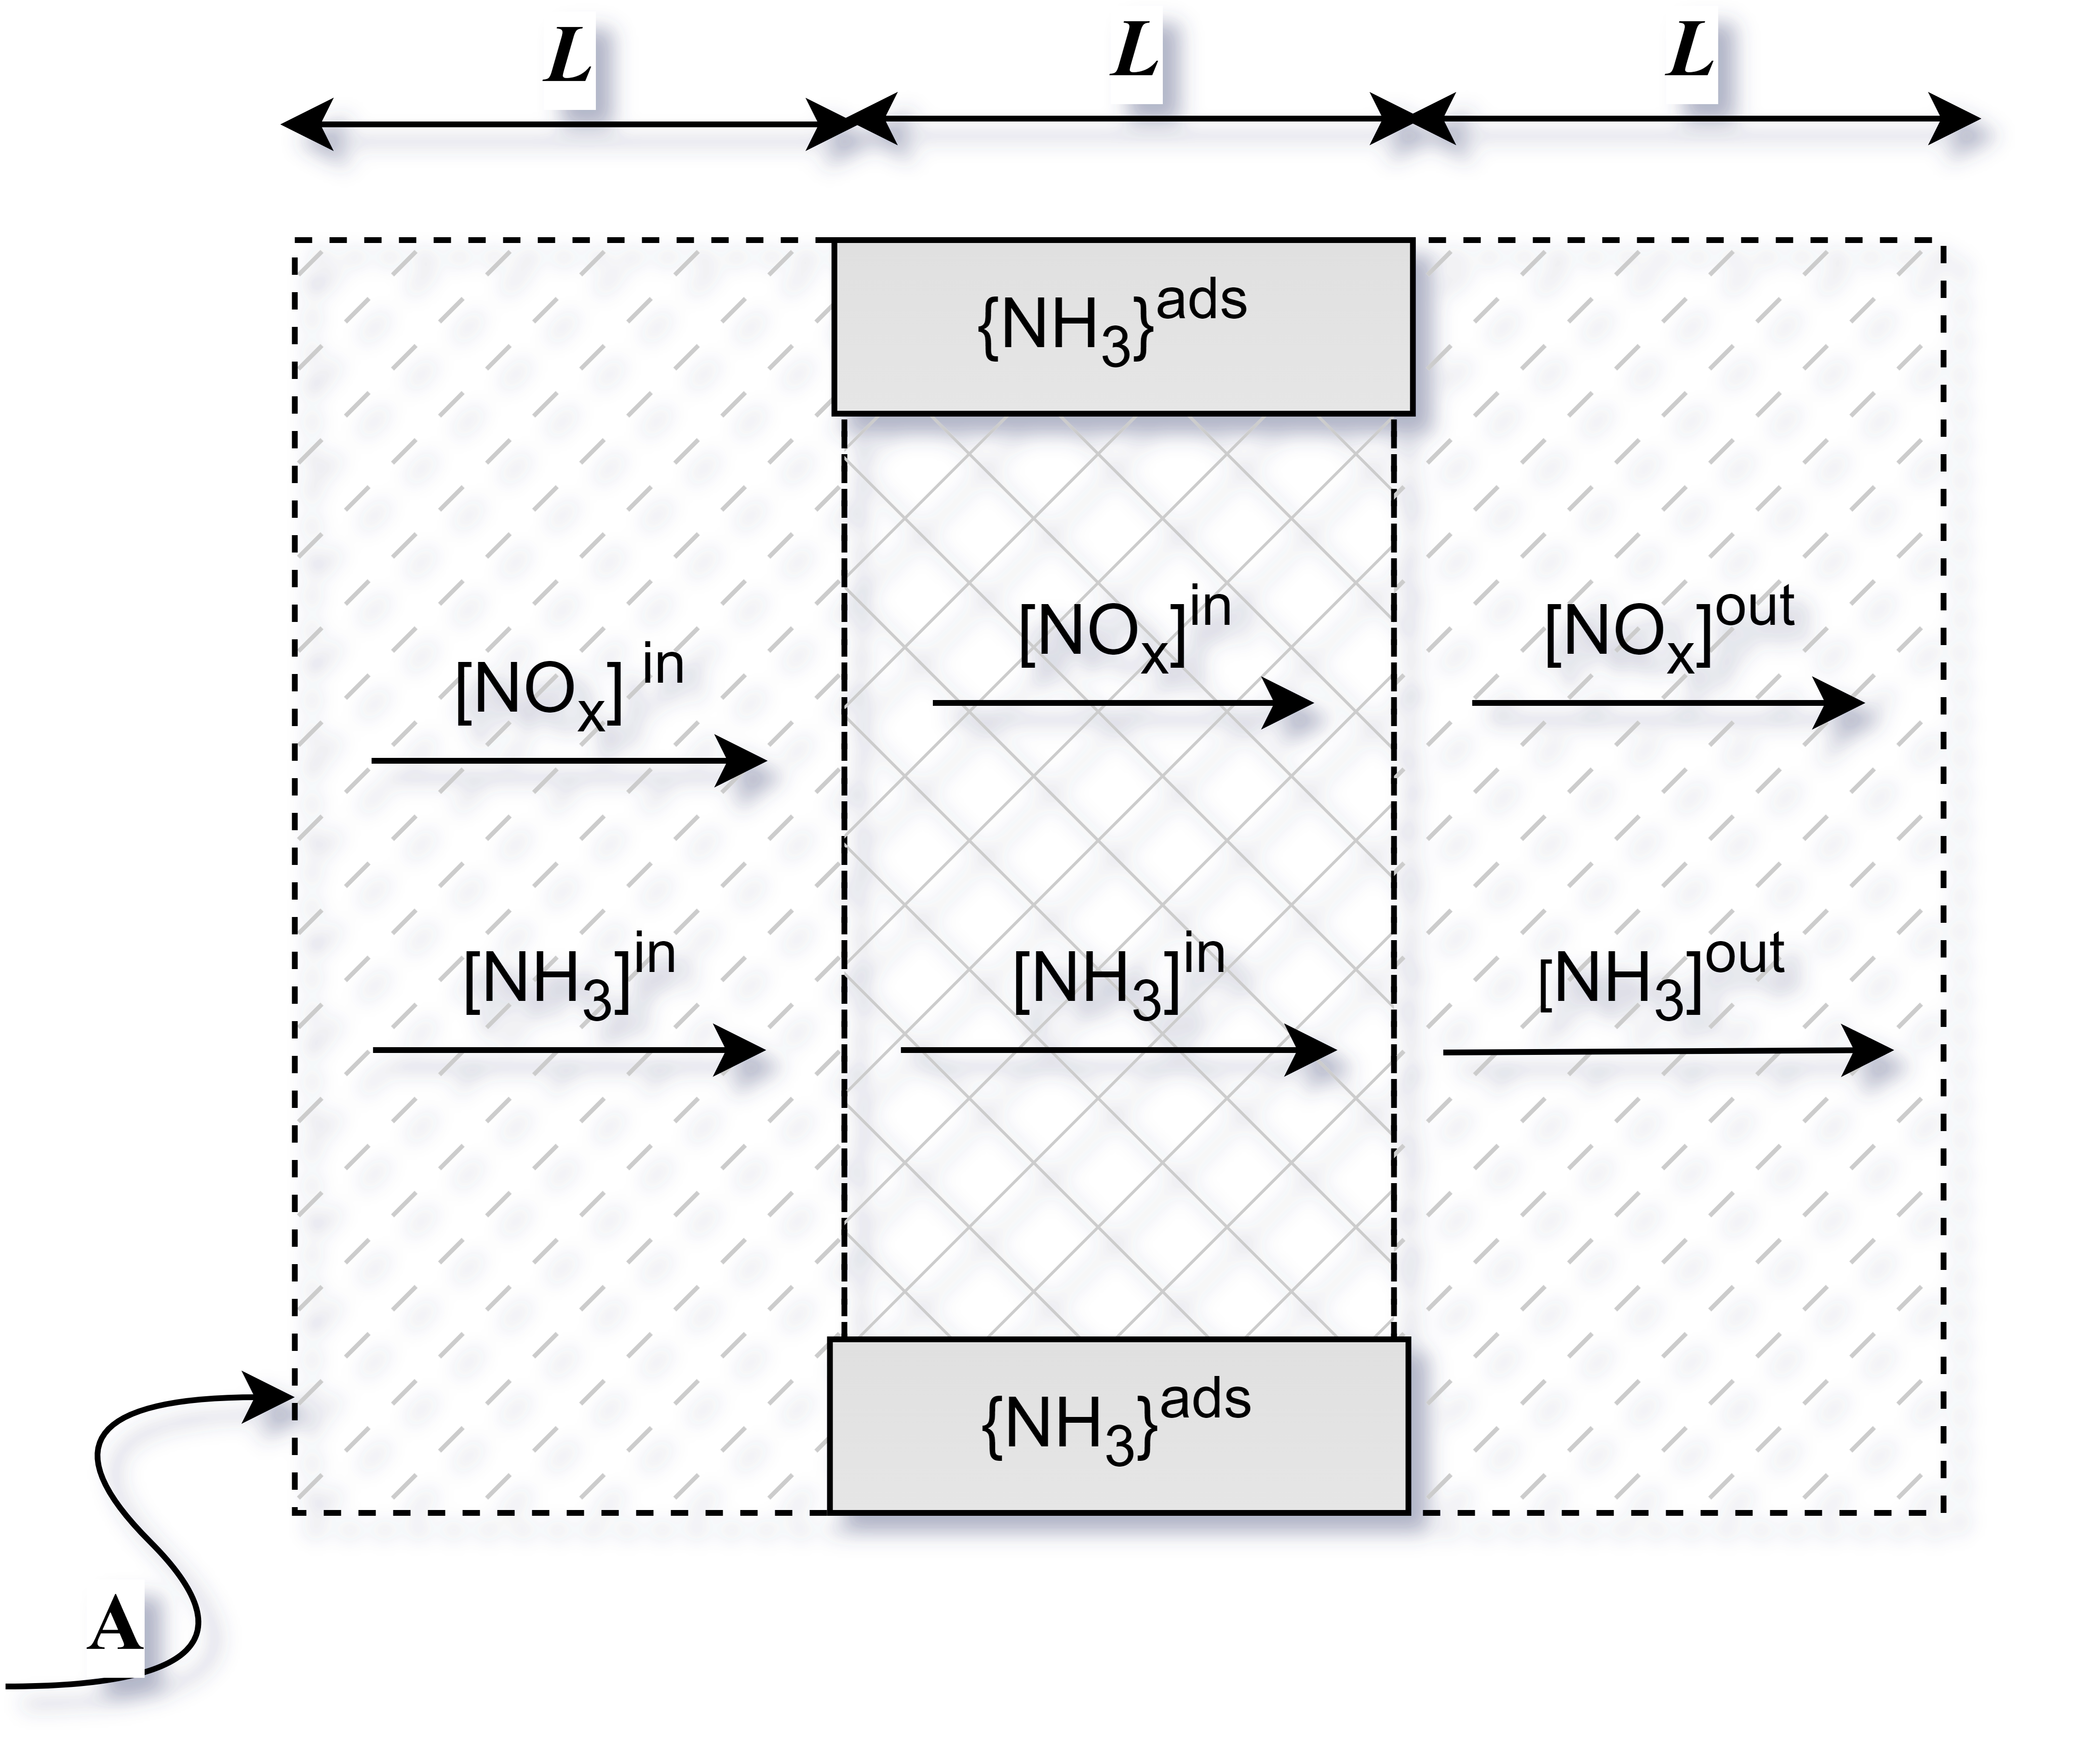
\includegraphics[width = 0.5\textwidth]{./figs/scr_sys/plug_flow_discrete.png}
        \caption{SCR-ASC system abstraction}
\end{figure}
\begin{enumerate}
        \item We have the molar-conservation equations across the control volume within one residence time.
                \begin{multline}
                        \underbrace{\mol{NO_x}^{out} }_{ \con{NO_x}^{out} \tau F_{vol} } (t + (i+1) \tau) =
                                \underbrace{\mol{NO_x}^{in} }_{ \con{NO_x}^{in} \tau F_{vol} } (t + i \tau)
                                + V_{scr} \int_0^{\tau}
                                                \underbrace{\frac{d}{dt} \con{NO_x}^{scr}}_
                                                        {k_{s2v} k_{scr} \con{NO_x}^{in} \con{NH_3}^{ads}}
                                           dt
                        \label{eqn::nox_bal}
                \end{multline}
                \begin{multline}
                       \mol{NH_3}^{ads} (t + (i+1) \tau) =
                                \underbrace{\mol{NH_3}^{ads} }_{A_{scr} \con{NH_3}^{ads}} (t + i \tau)
                                + A_{scr} \int_0^{\tau}
                                               \frac{d}{dt} \con{NH_3}^{ads}
                                               % \underbrace{}_{
                                               %         - \con{NH_3}^{ads}
                                               %                \lrf{
                                               %                k_{ads} \con{NH_3}^{in}
                                               %                + k_{scr} \con{NO_x}^{in}
                                               %                + k_{od}}
                                               %         + \Gamma k_{ads} \con{NH_3}^{in}
                                               %                }
                                                dt
                        \label{eqn::ads_bal}
                \end{multline}
        \item By summing the equations from (\ref{eqn::nox_bal}) for  $i = 0$ to $n-1$, where $n$ is the total number of residence times within one sampling period $(= t_s/\tau)$, we get the relation between the total moles of $NO_x$ that entered, reduced and left the SCR-ASC chamber. Finally, writing the equation in-terms of the inlet and outlet concentrations we get the equation relating inlet and outlet concentrations at the end of sampling period as:
                \begin{multline}
                        \underbrace{\con{NO_x}^{in}}_{x_1}(t + t_s) =
                                \underbrace{\con{NO_x}^{in}}_{u_1}(t) + \tau(t) k_{s2v} k_{scr}(t) \con{NO_x}^{in}(t) \underbrace{\lrf{\frac{1}{n} \sum_{i = 0}^{n-1} \con{NH_3}^{ads}(t + i \tau)}}_{\sigma}
                        \label{eqn::nox_avg}
                \end{multline}

        \item The dynamics of $\sigma$, the average surface concentration of adsorbed ammonia on the catalyst for the given sampling period, can be obtained by summing the equations from (\ref{eqn::ads_bal}) for $i = 0$ to $n-1$ which is the sampling period. This results in a telescopic cancellation of the terms resulting in an equation relating the moles in the current sample to the moles in the next sample. We have,
                \begin{multline}
                        \sigma(t + t_s) = \sigma(t) - \sigma(t) t_s \lrf{k_{ads}(t) \con{NH_3}^{in}(t)
                                                                                + k_{scr}(t) \con{NO_x}^{in}(t)
                                                                                + k_{od}(t)}
                                                \\
                                                + \Gamma t_s k_{ads}(t) \con{NH_3}^{in}(t)
                        \label{eqn::ads_avg}
                \end{multline}
        \item Finally, using (\ref{eqn::nox_avg}), $\sigma(t+ts), \sigma(t)$ can be eliminated from (\ref{eqn::ads_avg}) for getting a dynamic model for $NO_x$-reduction process which explicitly depends on the measured inputs and states alone.
                \begin{align}
                        \text{Let, }\quad \eta(k) = u_1(k-1) - x_1(k)
                \end{align}
                \begin{multline}
                        \eta(k + 1) = \eta(k) \lrb{\frac{\tau(k)}{\tau(k-1)}} \lrb{\frac{u_1(k)}{u_1(k-1)}} \\
                                        - t_s \eta(k) \lrb{\frac{\tau(k)}{\tau(k-1)}}
                                        \left\{ \lrb{\frac{u_1(k)}{u_1(k-1)}} k_{ads}(k-1) \con{NH_3}^{in}(k-1)
                                           \right.
                                        \\ \left. + \lrb{\frac{u_1(k)}{u_1(k-1)}} k_{od}(k-1)
                                                  + k_{scr}(k) u_1 (k)\right\}
                                        \\ + t_s k_{s2v} \Gamma \tau(k) \lrf{k_{scr}(k) k_{ads}(k-1)} u_1(k) \con{NH_3}^{in} (k-1)
                \label{eqn::disc_NOx}
                \end{multline}
\end{enumerate}

The above equation (\ref{eqn::disc_NOx}) is parametrized using the models for the physical properties and
urea-dosing and used for parameter estimation and validation.

Steps, 1, 2 and 3 are discussed in detail in the previous sections. The step-4 derivation is presented below followed by the parametrization.


\subsection{Modelling using average concentration change of $NO_x$ in a sample}
$\eta$ denote the change in concentration from the inlet to outlet in the $NO_x$ in one sample. This is the change in concentration in the exhaust due to the $NO_x$ reduction.
%
\begin{align}
        \eta(k) &= \con{NO_x}^{in}(k-1) - \con{NO_x}^{out}(k) = u_1(k-1) - x_1(k)
\end{align}
%
Thus, rewriting the $NO_x$ process dynamics (\ref{eqn::nox_avg}) interms of $\eta$, we have,
\begin{align}
        \eta(k+1) &= \tau(k) k_{s2v} k_{scr}(k) u_1(k) \sigma(k)\\
        %===
        \implies \sigma(k) &= \frac{\eta(k+1)}{\tau(k) k_{s2v} k_{scr}(k) u_1(k)}
        \label{eqn::sigma_elim}
\end{align}
%
The above equation (\ref{eqn::sigma_elim}) can be used to eliminate the unknown quantity $(\sigma)$ from equation (\ref{eqn::ads_avg}). We have,
\begin{multline}
        \sigma(k+1) = \sigma(k) - \sigma(k) t_s k_{ads}(k) \con{NH_3}^{in}(t)
                        - \sigma(k) t_s k_{scr}(k) u_1(k)
                        - \sigma(k) t_s k_{od}(k)
                        \\ + \Gamma(k) t_s k_ads(k) \con{NH_3}^{in}(k)
\end{multline}
writing the above equation for $\sigma(k)$:
\begin{multline*}
         \sigma(k) = \sigma(k-1)\lrf{1 -  t_s k_{ads}(k-1) \con{NH_3}^{in}(t-1)
                        -  t_s k_{scr}(k-1) u_1(k-1)
                        -  t_s k_{od}(k-1)}
                        \\ + \Gamma(k-1) t_s k_{ads}(k-1) \con{NH_3}^{in}(k-1)
\end{multline*}
Let,
\begin{align}
        \gamma_{proc}(k-1) &= \lrf{1 -  t_s k_{ads}(k-1) \con{NH_3}^{in}(t-1)
                        -  t_s k_{scr}(k-1) u_1(k-1)
                        -  t_s k_{od}(k-1)}
\end{align}
Using equation (\ref{eqn::sigma_elim}),
\begin{multline*}
        \frac{\eta(k+1)}{\tau(k) k_{s2v} k_{scr}(k) u_1(k)}
        = \frac{\eta(k)}{\tau(k-1) k_{s2v} k_{scr}(k-1) u_1(k-1)} \times \gamma_{proc}(k-1)\\
                        \\ + \Gamma(k-1) t_s k_{ads}(k-1) \con{NH_3}^{in}(k-1)
\end{multline*}
Thus, we have the recursive equation for change in concentration due to reduction:
\begin{multline}
        \eta(k+1) = \eta(k) \times \lr{\frac{\tau(k)}{\tau(k-1)}}
                                \times \lr{\frac{u_1(k)}{u_1(k-1)}}
                                \times \lr{\frac{k_{scr}(k)}{k_{scr}(k-1)}}
                                \times \gamma_{proc}(k-1)
                                \\
                        + t_s k_{s2v} \times \lrf{\Gamma(k-1) \tau(k) u_1(k)} \times \lr{k_{scr}(k) k_{ads}(k-1)}
\end{multline}
Explicitly writing the individual terms:
\begin{align*}
        \eta(k+1) =& \eta(k) \lrb{\frac{\tau(k)}{\tau(k-1)}}
                                \lrb{\frac{u_1(k)}{u_1(k-1)}}
                                \lrb{\frac{k_{scr}(k)}{k_{scr}(k-1)}} \\
                &-\eta(k) \lrb{\frac{\tau(k)}{\tau(k-1)}}
                                \lrb{\frac{u_1(k)}{u_1(k-1)}}
                                \lrb{\frac{k_{scr}(k)}{k_{scr}(k-1)}}
                t_s k_{ads}(k-1) \con{NH_3}^{in}(t-1)
                \\
                &-\eta(k) \lrb{\frac{\tau(k)}{\tau(k-1)}}
                                \lrb{\frac{u_1(k)}{u_1(k-1)}}
                                \lrb{\frac{k_{scr}(k)}{k_{scr}(k-1)}}
                t_s k_{scr}(k-1) u_1(k-1)
                \\
                &-\eta(k) \lrb{\frac{\tau(k)}{\tau(k-1)}}
                                \lrb{\frac{u_1(k)}{u_1(k-1)}}
                                \lrb{\frac{k_{scr}(k)}{k_{scr}(k-1)}}
                t_s k_{od}(k-1)
                \\
                &+ t_s k_{s2v} \times \lrf{\Gamma(k-1) \tau(k) u_1(k)} \times \lr{k_{scr}(k) k_{ads}(k-1)}
\end{align*}
The above equation can be simplified using the following two assumptions:
\begin{itemize}
        \item[$A1.$] The temperature doesn't change significantly across contiguous samples, i.e., $T(k-1) \approx T(k)$.
        \begin{align}
                \implies \frac{k_{scr}(k)}{k_{scr}(k-1)} \approx 1
        \end{align}
        \item[$A2.$] The product of rate constants results in a combined rate-constant,
        \begin{align}
                k_{scr}(k) k_{ads}(k-1) &\approx k_{scr}(k-1) k_{ads}(k-1)  = A_{scr}A_{ads} \exp\lrf{\frac{E_{scr}+E_{ads}}{R T(k-1)}} = k_{scr/ads}(k-1)
        \end{align}
\end{itemize}
Incorporating the above assumptions we have the dynamic model for change in concentration due $NO_x$ reduction:
\begin{align*}
         \eta(k+1) =& \eta(k) \lrb{\frac{\tau(k)}{\tau(k-1)}}
                                \lrb{\frac{u_1(k)}{u_1(k-1)}}
                \\
                &-\eta(k) \lrb{\frac{\tau(k)}{\tau(k-1)}}
                                \lrb{\frac{u_1(k)}{u_1(k-1)}}
                t_s k_{ads}(k-1) \con{NH_3}^{in}(t-1)
                \\
                &-\eta(k) \lrb{\frac{\tau(k)}{\tau(k-1)}}
                t_s k_{scr}(k) u_1(k)
                \\
                &-\eta(k) \lrb{\frac{\tau(k)}{\tau(k-1)}}
                                \lrb{\frac{u_1(k)}{u_1(k-1)}}
                t_s k_{od}(k-1)
                \\
                &+ t_s k_{s2v} \times \lrf{\Gamma(k-1) \tau(k) u_1(k)} \times k_{scr/ads}(k-1)
\end{align*}
\begin{equation}
       \label{eqn::nox_govern}
\end{equation}

